% Software ontwerp
\chapter{Softwareontwerp}\label{chapter:softwareontwerp}


%%%%%%%%%%%%%%%%%%%%%%%%%%%%%%%%%%%%%%%%%%%%%%
% SECTION Data model
%%%%%%%%%%%%%%%%%%%%%%%%%%%%%%%%%%%%%%%%%%%%%%
\section{Datamodel}\label{section:data_model}

Beide applicaties maken gebruik van hetzelfde datamodel. Het is een eenvoudige tabel in een SQLite database zoals te zien in tabel \ref{tab:qdat}. SQLite is relatief eenvoudig te integreren in beide technologie\"en\footnote{SQLite tutorial voor iOS: \cite{techotopia2012sqlite}, SQLite tutorial voor Android: \cite{android2013sqlite}}. De SQL-code om een database en tabellen aan te maken en te verwijderen is uiteraard hetzelfde.

\begin{table}[h]
\caption{QDat SQLite Table}
\begin{center}
	\begin{tabular}{ l l } % l = left-aligned column
		\hline
		\textbf{QDat}		&									\\
		\hline
		id (pk)					&		INTEGER 			\\
		date 						&		TIMESTAMP 		\\
		work\_quantity	&		REAL[0, 24]		\\
		work\_quality		&		INTEGER[0..2]	\\
		mood\_quantity	&		REAL[0, 10]		\\
		\hline
	\end{tabular}
\end{center}
\label{tab:qdat}
\end{table}

Een andere mogelijkheid, specifiek voor iOS, is het gebruik van Core Data. Met dit framework kan dataopslag gebeuren aan de hand van een object-geori\"enteerde abstractielaag\cite{techotopia2012coredata}. Voor deze relatief kleine applicatie volstaat een SQLite database echter.



%%%%%%%%%%%%%%%%%%%%%%%%%%%%%%%%%%%%%%%%%%%%%%
% SECTION Structuur
%%%%%%%%%%%%%%%%%%%%%%%%%%%%%%%%%%%%%%%%%%%%%%
\section{Structuur}\label{section:structuur}

De projectstructuur voor de twee projecten verschilt weinig in grote lijnen. Het aantal schermen is hetzelfde, net als het aantal controllers. Het model voor de Android-applicatie is iets uitgebreider dan in de iOS-versie, maar dit is eerder een gevolg van de manier waarop de database werd ge\"implementeerd, dan de constraints van de technologie zelf.


%%%%%%%%%%%%%%%%%%%%
%			 Android
%%%%%%%%%%%%%%%%%%%%
\subsection{Android}

De Android-app is opgebouwd uit vier klassen die overerven van de \textit{Activity}-klasse, met bijbehorende XML-files voor de views zoals te zien in tabel \ref{tab:android_activities}. \textit{HomeActivity} is het startpunt van de applicatie. Het scherm toont twee knoppen: \'e\'en om te navigeren naar de \textit{QWorkActivity} pagina en \'e\'en om de resultatenpagina, \textit{DataVisActivity}, te laden. De view van \textit{QWorkActivity} bevat enkele labels, een invoerveld, een radioboxgroep en een knop om naar \textit{QMoodActivity} te navigeren. In de view van \textit{QMoodActivity} staat er een label, een slider en een knop om naar \textit{HomeActivity} terug te keren. Hierbij wordt eveneens de data gepersisteerd in de SQLite databank.

\begin{table}[h]
\caption{Android Activity klassen met bijbehorende XML-files}
\begin{center}
	\begin{tabular}{ l l } % l = left-aligned column
		\hline
		\textbf{Activity}								&	\textbf{XML}											\\
		\hline
		\textit{HomeActivity}.java			&	\textit{activity\_home}.xml 			\\
		\textit{QWorkActivity}.java			&	\textit{activity\_qwork}.xml			\\
		\textit{QMoodActivity}.java 		&	\textit{activity\_qmood}.xml 			\\
		\textit{DataVisActivity}.java		&	\textit{activity\_data\_vis}.xml	\\
		\hline
	\end{tabular}
\end{center}
\label{tab:android_activities}
\end{table}

Om de connectie met de database te maken, wordt er gebruik gemaakt van een implementatie van de SQLiteOpenHelper-klasse; de klasse \textit{DatabaseHandler} in dit project. De klasse \textit{CRUD<E>} is een templateklasse voor het beheren van een database tabel. Deze heeft de typische methodes \textit{createTable}, \textit{dropTable}, \textit{insert}, \textit{delete}, \textit{update} en \textit{select}.

De modelklasse \textit{QDat} implementeert de \textit{Parcelable} interface. Dit zorgt ervoor dat we op een effici\"ente manier objecten tussen \textit{Activity}-klassen kunnen doorgeven.

Het volledige klassediagram voor de Android-applicatie is te zien op figuur \ref{fig:android_classdiagram}.

\begin{figure}
  \begin{center}
  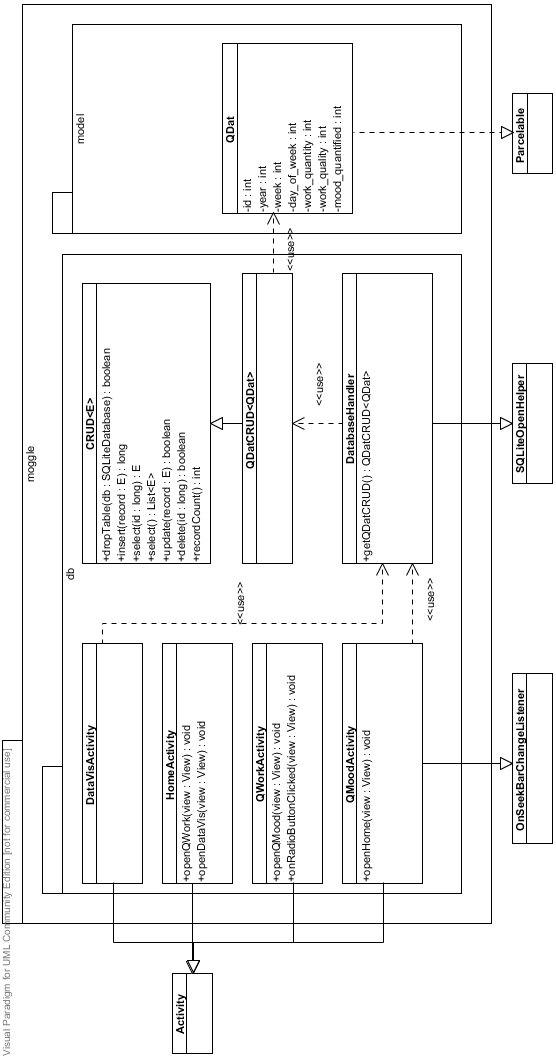
\includegraphics[scale=0.7]{data/diagram-android}
	\end{center}
  \caption{Android Class Diagram van de Moggle applicatie}
  \label{fig:android_classdiagram}
\end{figure}


%%%%%%%%%%%%%%%%
%			iOS
%%%%%%%%%%%%%%%%
\subsection{iOS}

Het ontwerpen van de iOS-app is grotendeels gebaseerd op het storyboard. Er zijn vier views met bijbehorende \textit{UIViewController}-implementaties: \textit{ViewController}, \textit{QWorkController}, \textit{QMoodController} en \textit{ResultsController}.

De UI-elementen komen grotendeels overeen met die van de Android-versie. Behalve in de view van de \textit{QWorkController}: de stepper biedt een mooie voorgedefinieerde functionaliteit om op een eenvoudige manier een natuurlijk getal in te geven door de huidige waarde met stappen van \'e\'en te verhogen of te verlagen.

Een interessante eigenschap van iOS is het doorgeven van argumenten tussen controllers van opeenvolgende views. Het volstaat hierbij in de methode \textit{prepareForSegue} de pointer naar het object expliciet te initialiseren in de targetcontroller.

Het klassediagram voor de iOS-applicatie is te zien op figuur \ref{fig:ios_classdiagram}. %Figuur \ref{fig:ios_storyboard} toont het storyboard van de iOS-applicatie.

\begin{figure}
  \begin{center}
  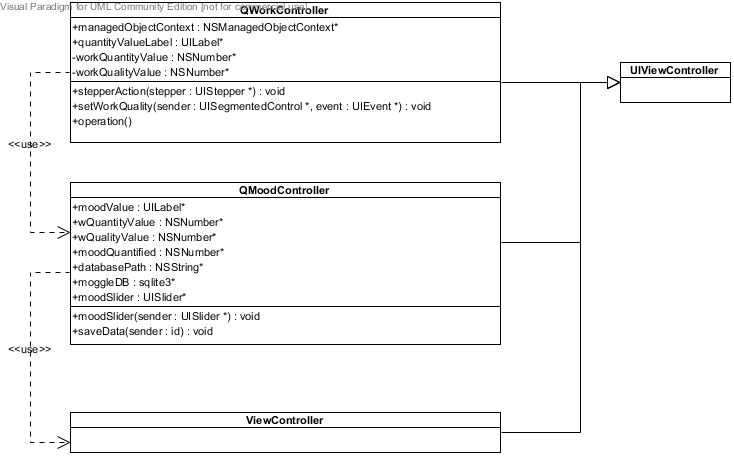
\includegraphics[scale=0.7]{data/diagram-ios}
	\end{center}
  \caption{iOS Class Diagram van de Moggle applicatie}
  \label{fig:ios_classdiagram}
\end{figure}

%\begin{figure}
%  \begin{center}
%  
\includegraphics[scale=0.7]{data/ios-storyboard}
%	\end{center}
%  \caption{iOS storyboard van de Moggle applicatie}
%  \label{fig:ios_storyboard}
%\end{figure}



%%%%%%%%%%%%%%%%%%%%%%%%%%%%%%%%%%%%%%%%%%%%%%
% SECTION Structuur
%%%%%%%%%%%%%%%%%%%%%%%%%%%%%%%%%%%%%%%%%%%%%%
\section{Uitbreidingen}\label{section:uibreidingen}

Mogelijke uitbreidingen aan de huidige applicaties zouden bijvoorbeeld de volgende kunnen zijn:

\begin{itemize}
	\item dataopslag gecentraliseerd op een server;
	\item	integratie met de Toggl API;
	\item	implementatie van verschillende data visualisaties;
	\item een notificatiesysteem uitbouwen op basis van gebruikersvoorkeuren;
	\item	combinatie met Google Calendar: afhankelijk van de weekplanning notificaties sturen;
	\item	...
\end{itemize}

Al bij al is het nog maar een zeer klein project, dus echt grote ontwerpbeslissingen hoefden nog niet genomen te worden. Door de applicatie enkel voor iPhone te ontwikkelen en niet voor bijvoorbeeld de iPad, worden bovendien een deel van de mogelijke problemen uitgesloten, gerelateerd aan de layout van de schermen en visualisaties.

% mogelijke uitbreidingen in de toekomst
% mogelijke veranderingen aan het huidige systeem









